
\begin{figure}[H]
	\centering
	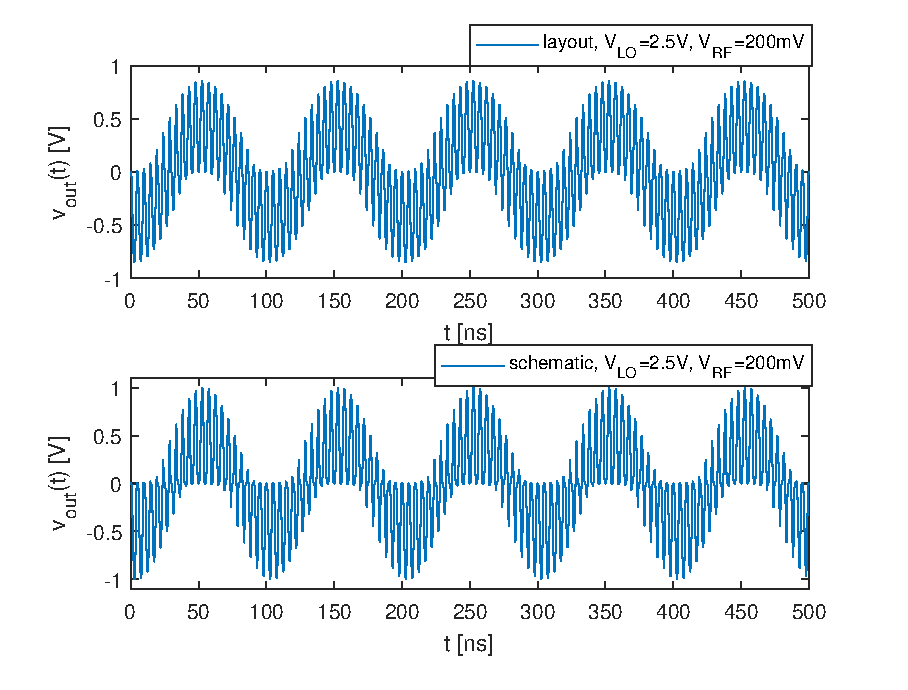
\includegraphics[scale=0.7]{waveforms}
	\caption{Time domain waveforms: double balanced differential output with v\textsubscript{RF}=200mV,  f\textsubscript{RF}=110MHz, v\textsubscript{RF}=1.23mV, f\textsubscript{LO}=100MHz.}
	\label{fig:TdomaniWF}
\end{figure}


\section{Simulation vs schematic comparison}

Last step was to characterize the layout and evaluate its behaviour in comparison with the schematic. The analysis carried on are the following:
\begin{itemize}
	\item Time domain mixed signal and spectral components
	\item Oscillator amplitude to maximize output component
	\item Conversion gain and 1dB compression point
	\item Single tone IIP\textsubscript{3}
	\item Two tone IIP\textsubscript{3}
	\item Bandwidth and CMRR of RF stage (output node filtering of output signal, current mixing)
	\item Static power dissipation
\end{itemize}
All the analysis were developed using monochromatic signals at frequencies 100MHz for LO, 110MHz for RF, and considering the mixer working in down-conversion (10MHz IF frequency).

\begin{figure}[H] 
	\centering
	\subfloat[][\emph{layout}]{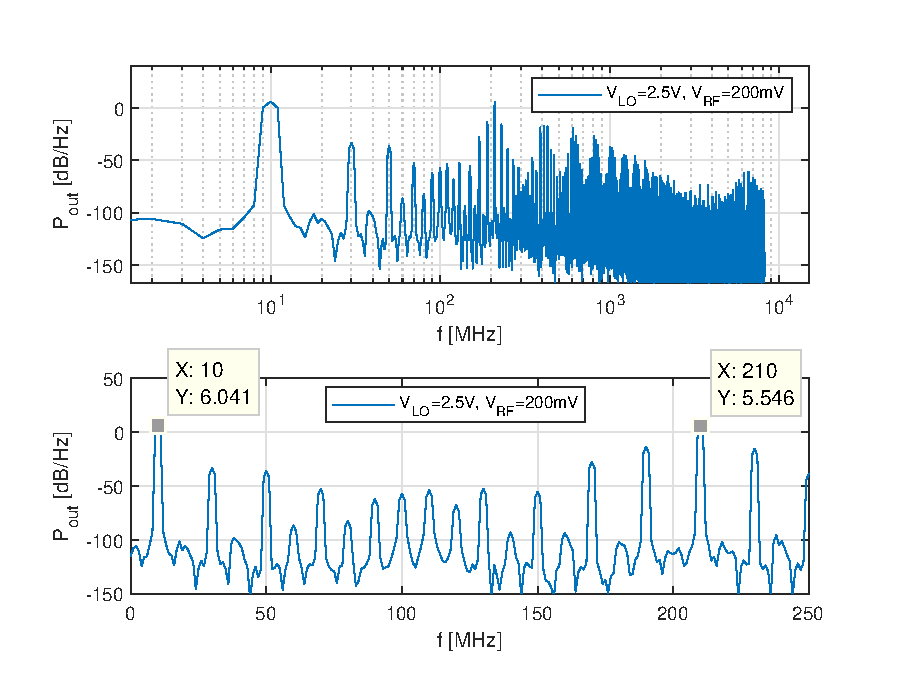
\includegraphics[scale=.6]{DFT_layout}} \\
	\subfloat[][\emph{schematic}]{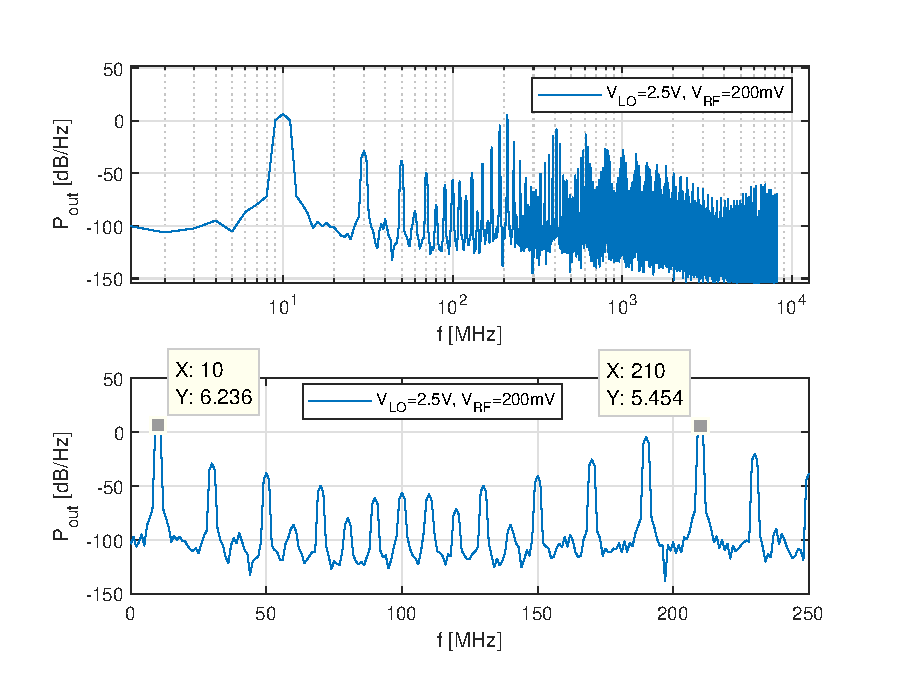
\includegraphics[scale=.6]{DFT_schem}}
	\caption{Discrete Fourier transform: double balanced differential output with v\textsubscript{RF}=200mV,  f\textsubscript{RF}=110MHz, v\textsubscript{RF}=1.23mV, f\textsubscript{LO}=100MHz,cosine squared smoothing function. a) layout, b) schematic}
	\label{fig:TdomaniDFT}
\end{figure}
\subsection{Time domain mixed signal}
The mixed output signal with \(v_{rf}=\)200mV and \(v_{lo}=\)1.23V is visible in figure \ref{fig:TdomaniWF}. The waveform looks like the expected one from literature \textbf{(REFERENCE)}.
Applying the discrete Fourier transform to the if signal we found the graph seen in figure \ref{fig:TdomaniDFT}a and \ref{fig:TdomaniDFT}b.
It's clearly visible the intrinsic capability of double balanced mixer of rejecting input components at \(v_{lo}=100\)MHz and \(v_{rf}=\)110MHz.

\begin{figure}[H]
	\centering
	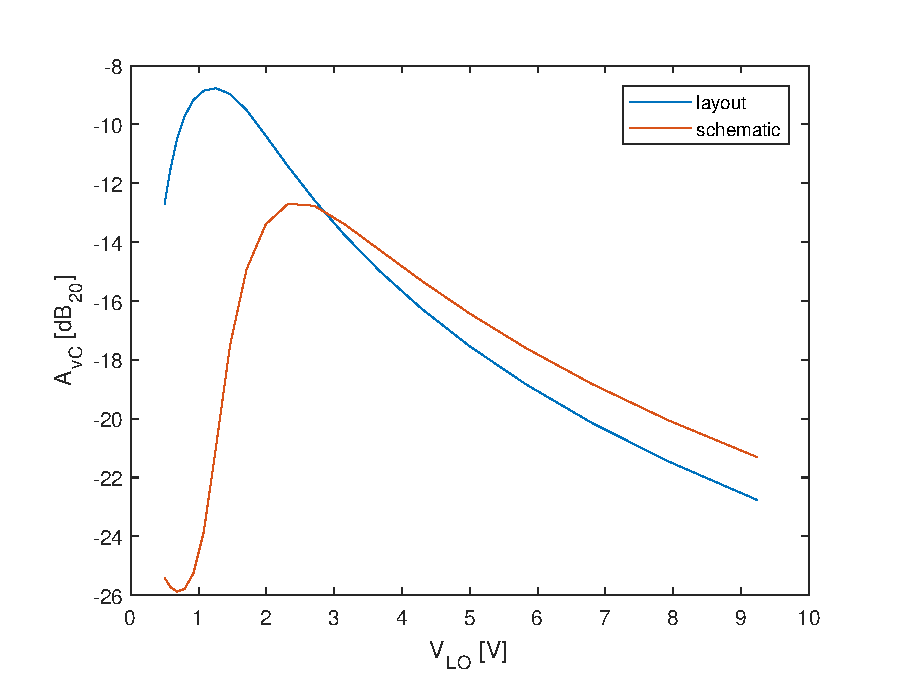
\includegraphics[scale=0.7]{gain_vs_VLO}
	\caption{Conversion gain vs v\textsubscript{LO}.}
	\label{fig:maxGainvsLO}
\end{figure}

\subsection{Maximum conversion gain vs LO}
Input LO signal was swept to find the optimum value that maximizes output voltage at IF. The analysis has been carried on for both schematic and layout circuit. Voltage \(v_{rf}=200mV\) was kept constant during the analysis, and output amplitude at 10MHz was divided by LO amplitude such that the peak corresponds to the maximum LO amplitude for which IF output power saturates. Results are shown in figure \ref{fig:maxGainvsLO}. It can be noticed that schematic and layout reach their maximum for different values of LO signal, \(2.5V\) and \(1.23V\) respectively. In general it can be noticed that layout has an higher gain than the schematic. Trying to change \(v_{rf}\) amplitude very tiny changes in peak output voltage where found, so the first analysis was kept as a quite good estimation for optimum LO peak voltage. From now on all the comparison between the two circuits have been made imposing the optimum LO voltage for each circuit.


\subsection{Conversion gain and 1dB compression point}
Keeping optimum LO amplitude, RF's voltage was swept in order to see how output power at IF frequency increases with input power at RF. Reference port for all power measurement has been chosen to be \(50\ohm\). \(P_{IF}\) as a function of \(P_{RF}\) conversion gain is shown in figure \ref{fig:PinPout1T_1dBCp} for both schematic and layout, whereas gain can be seen in figure \ref{fig:GainvsRF}. 
\begin{figure}[H] 
	\centering
	\subfloat[][\emph{P\textsubscript{in}/P\textsubscript{out}}]{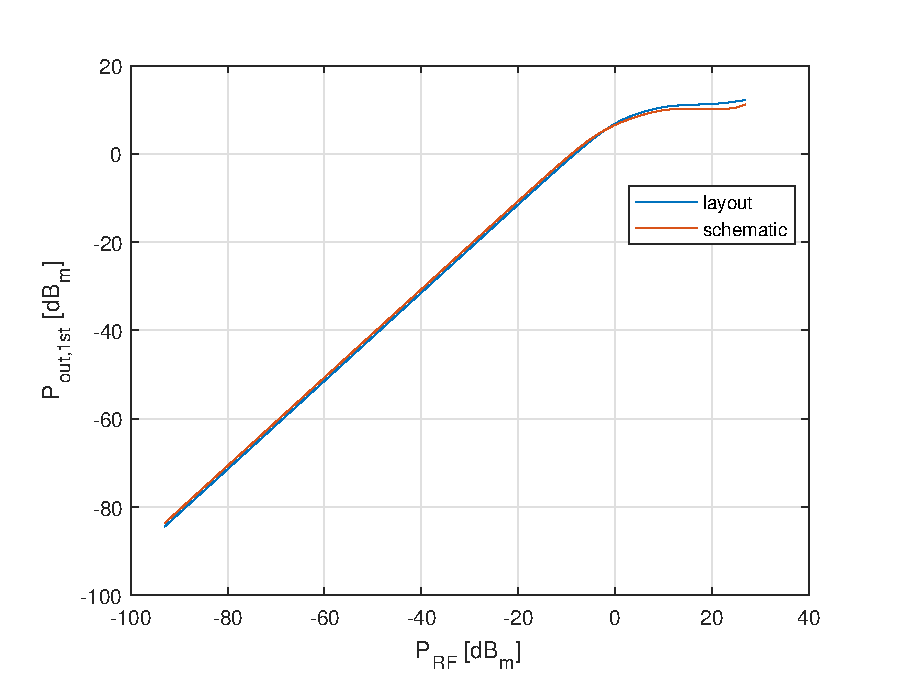
\includegraphics[scale=.7]{pin_pout_VRF}} \\
	\subfloat[][\emph{1dB compression point}]{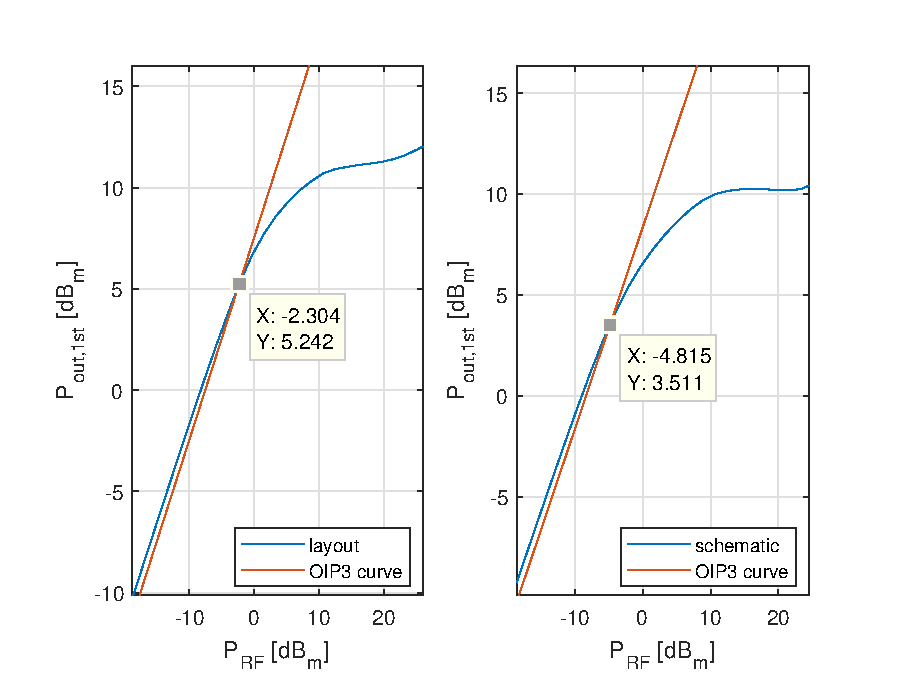
\includegraphics[scale=.7]{1dB_compression_1tone}}
	\caption{a) P\textsubscript{in}/P\textsubscript{out} and  b) 1dB compression point, one-tone analysis.}
	\label{fig:PinPout1T_1dBCp}
\end{figure}

From simulation we have:
\begin{gather}
G_C|_{layout}=4.27dB \Rightarrow A_{vC}|_{layout}=2.67 \notag \\ 
G_C|_{schematic}=4.88dB\Rightarrow A_{vC}|_{schematic}=3.08 \notag
\end{gather}
\begin{figure}[H]
	\centering
	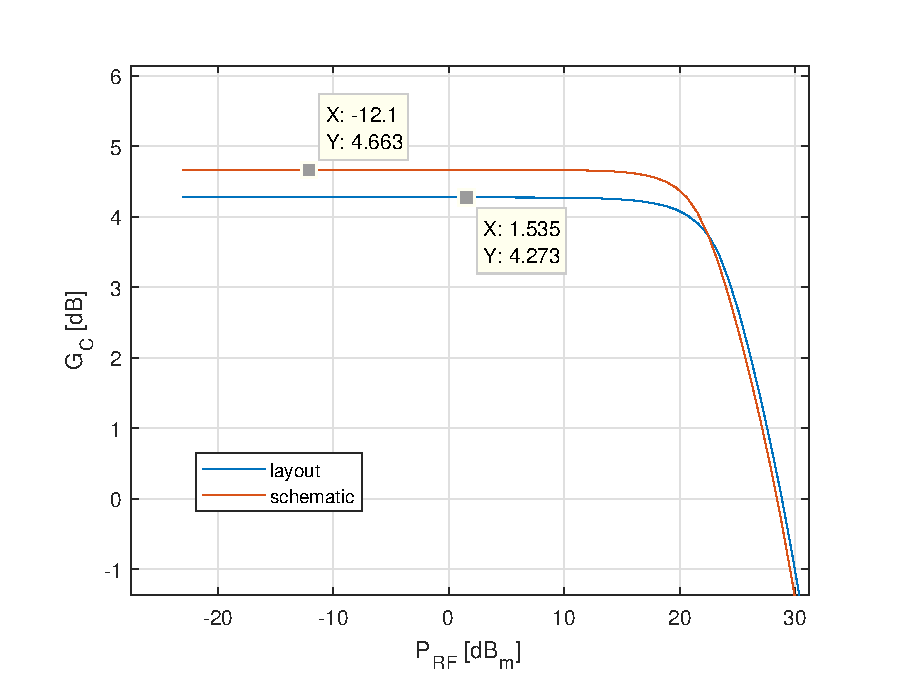
\includegraphics[scale=0.7]{gain_vs_VRF}
	\caption{Conversion gain vs v\textsubscript{RF}.}
	\label{fig:GainvsRF}
\end{figure}

Extrapolation of 1dB compression point was carried on, leading to the measurement of RF power for which the gain drops of 1dB equal to 
\begin{gather}
 P_{RF,in}|_{layout}=5.24dB_{m} \notag \\
 P_{RF,in}|_{schematic}=3.51dB_{m} \notag
\end{gather}
then, respectively for schematic and layout, corresponding to the voltages:
\begin{gather}
V_{RF,in}|_{layout}=122.3mV \notag \\
V_{RF,in}|_{schematic}=149.2mV \notag
\end{gather}

\subsection{Single tone third order distortion}
Using single tone RF signal, power on the third harmonic with respect to the IF tone has been measured. Third order distortion is in fact the first contribution to non-linearities\textbf{(SELFREFERENCE)}. 
The typical cubic behaviour with respect to the linear one of the conversion gain can be easily seen in logarithmic scale, shown in figure \ref{fig:IIP3_1t_schem} for the schematic and in figure \ref{fig:IIP3_1t_layout} for the layout. 
Linear regression was applied to the curves to find the third order intercept points for both schematic and layout test benches. Values of IIP3 and OIP3 thus found for both layout and schematic are reported in table \textbf{2}. From where it appears that the layout extracted introduces less third order distortion than schematic, fifth order distortion looks higher at lower input power though.

\begin{figure}[H] 
	\centering
	\subfloat[][\emph{harmonics power}]{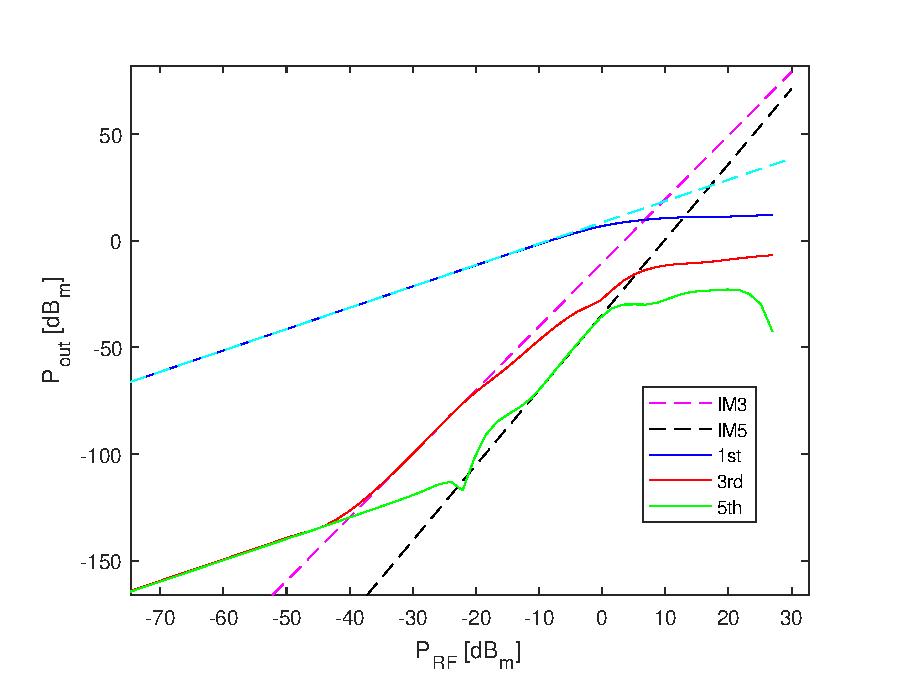
\includegraphics[scale=.7]{IIP3_schem_1tone}} \\
	\subfloat[][\emph{detail in IIP3 and IIP5}]{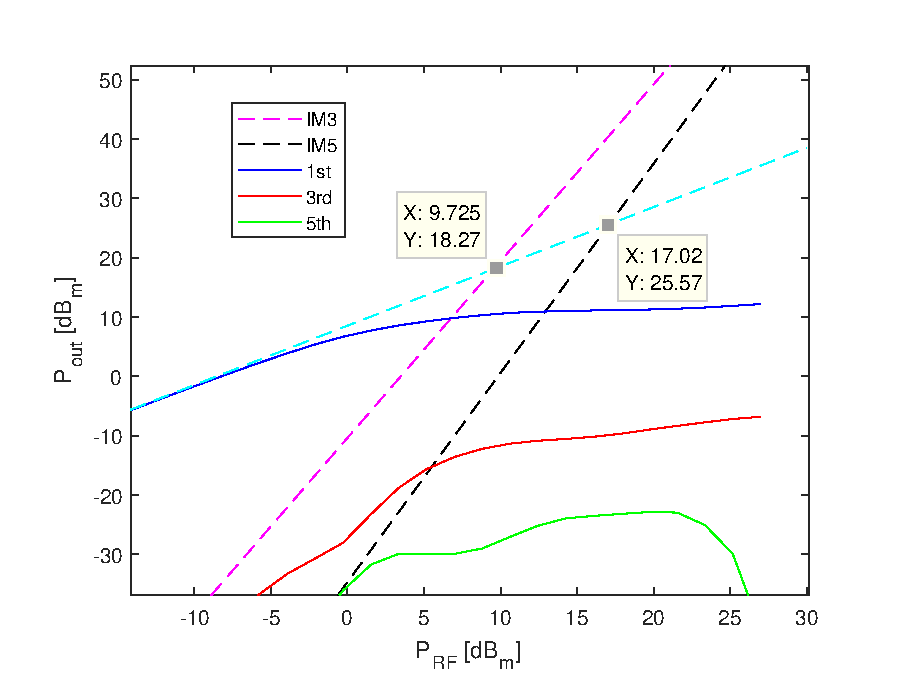
\includegraphics[scale=.7]{IIP3_schem_1tone_zoom}}
	\caption{Harmonics power, IIP\textsubscript{3} and IIP\textsubscript{5} in schematic, one tone analysis.}
	\label{fig:IIP3_1t_schem}
\end{figure}

\begin{figure}[H] 
	\centering
	\subfloat[][\emph{}]{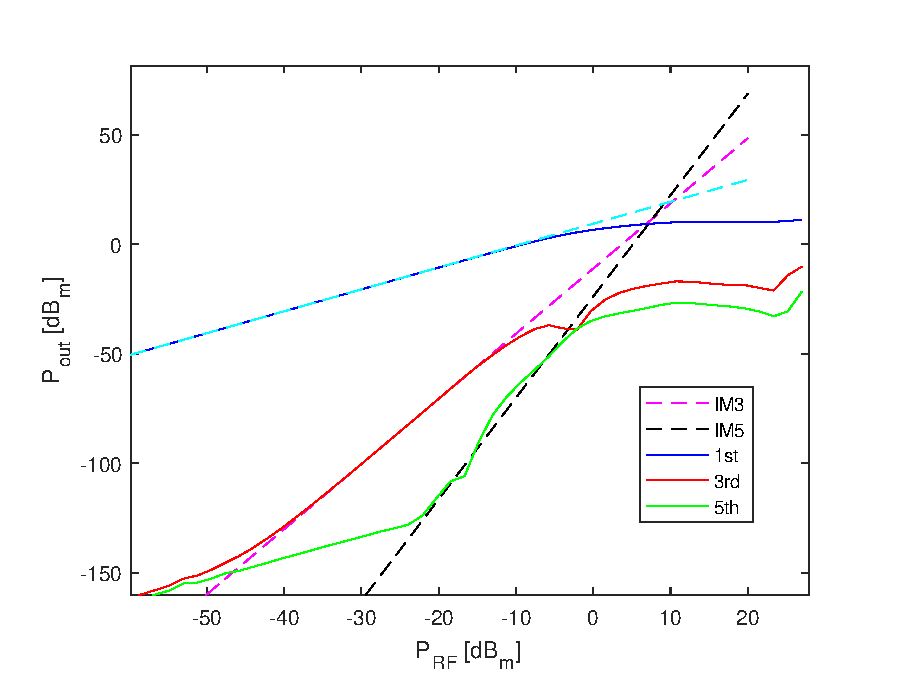
\includegraphics[scale=.7]{IIP3_layout_1tone}} \\
	\subfloat[][\emph{}]{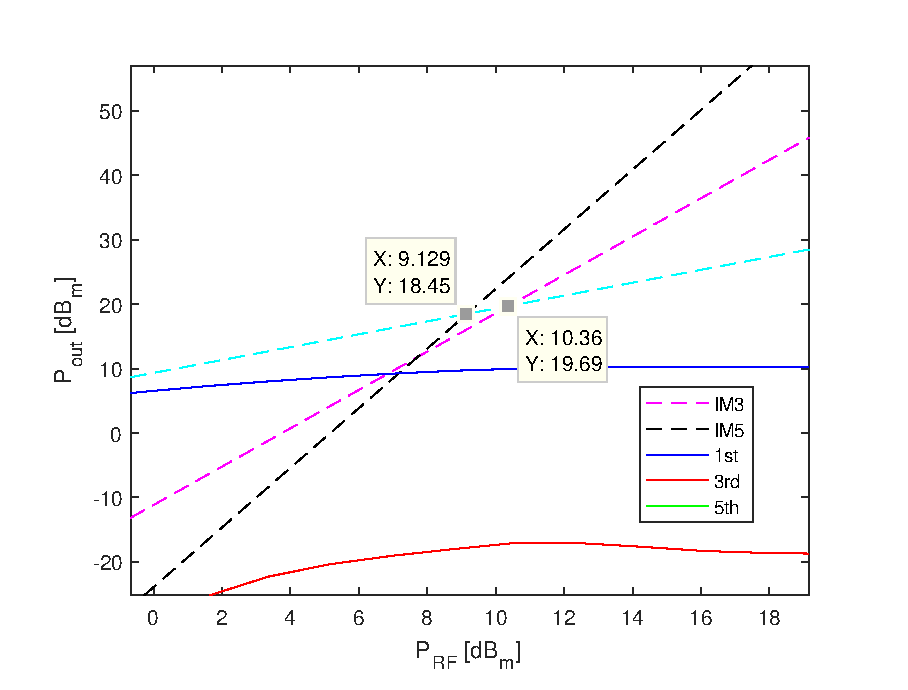
\includegraphics[scale=.7]{IIP3_layout_1tone_zoom}}
	\caption{IIP\textsubscript{3} and IIP\textsubscript{5} in layout, one tone analysis.}
	\label{fig:IIP3_1t_layout}
\end{figure}

\begin{table} [H]
	\label{tab:IIP3_1tone}
	\caption{IIP3 and IIP5 in one tone analysis.}
	\centering	
	\begin{tabular}{lccr} 
		\toprule 
		Parameter Name			& Schematic 	& Layout & unit \\ 
		\midrule
		\(IIP_{3}\)  & 9.73 & 10.4 & dB\(_{m}\) \\
		\(OIP_{3}\)  & 18.3 &19.7 & dB\(_{m}\) \\
		\(IIP_{5}\)  & 17.0 &9.13 & dB\(_{m}\) \\
		\(OIP_{5}\)  & 25.6 &18.5 & dB\(_{m}\) \\
		\bottomrule 
	\end{tabular}	
\end{table}
\subsection{Two tone IM\textsubscript{3} and CIM\textsubscript{3} ratio}
In order to simulate the behaviour of a non-monochrome, fixed-bandwidth signal, the two tone analysis has been carried on. Two RF tones at f\textsubscript{RF}=110MHz and f\textsubscript{RF}\textsuperscript{'}=f\textsubscript{RF}+\(\delta\)f=111MHz have been adopted.
Figure \ref{fig:1dB_2tones} shows the 1dB compression point in this case.
Third order intermodulation frequency components result to be at \(9Mhz\) and \(12MHz\). Their behaviour along with increasing input power is shown in figure \ref{fig:IIP3_2t_schem}a and \ref{fig:IIP3_2t_schem}b. 
Graphs show that power related to fundamental is strongly reduced when two tones are injected, since power is equally spread among them. From simulation appears that the IIP\textsubscript{3} is reduced by roughly three dB, accordingly to the doubled power injected due two tones. Once again the layout looks less performing. Frequency spectra at difference input power is shown in figure \ref{fig:DFT_2ton} and \ref{fig:DFT_2ton_zoom}. From the latter, informations about the carrier to third intermodulation data are selected. In particular, the 1dB compression point spectrum has been chosen (P\textsubscript{RF}=-9.68dB\textsubscript{m}), since this is set as the maximum input power accepted by the multiplier without heavy distortion. As it appears, power carried from fundamental tones (10MHz and 11MHz) barely increases after this point, whereas other tones keep increasing.

\begin{table} [H]
	\label{tab:IIP3_2tone}
	\caption{1dB compression point, IIP3 and CIM3 in two tones analysis.}
	\centering	
	\begin{tabular}{lccr} 
		\toprule 
		Parameter Name			& Schematic 	& Layout & unit \\ 
		\midrule
		\(P_{RF,1dB}\) & -8.01 & -9.68 & dB\(_{m}\)\\
		\(IIP_{3}\)  & 8.42 & 5.06 & dB\(_{m}\) \\
		\(OIP_{3}\)  & 16.9 &14.4 & dB\(_{m}\) \\
		\(CIM_{3,1dB}\) & 16.7 & 14.1 & dB \\
		\bottomrule 
	\end{tabular}	
\end{table}

\begin{figure}[H] 
	\centering
	\subfloat[][\emph{schematic}]{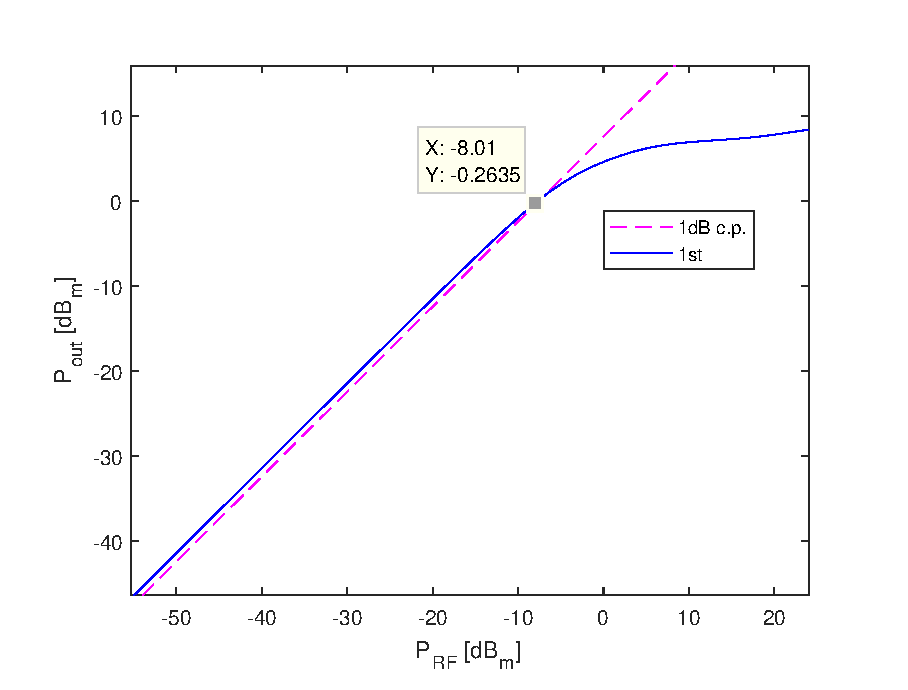
\includegraphics[scale=.7]{1dB_compression_2tone_schem}} \\
	\subfloat[][\emph{layout}]{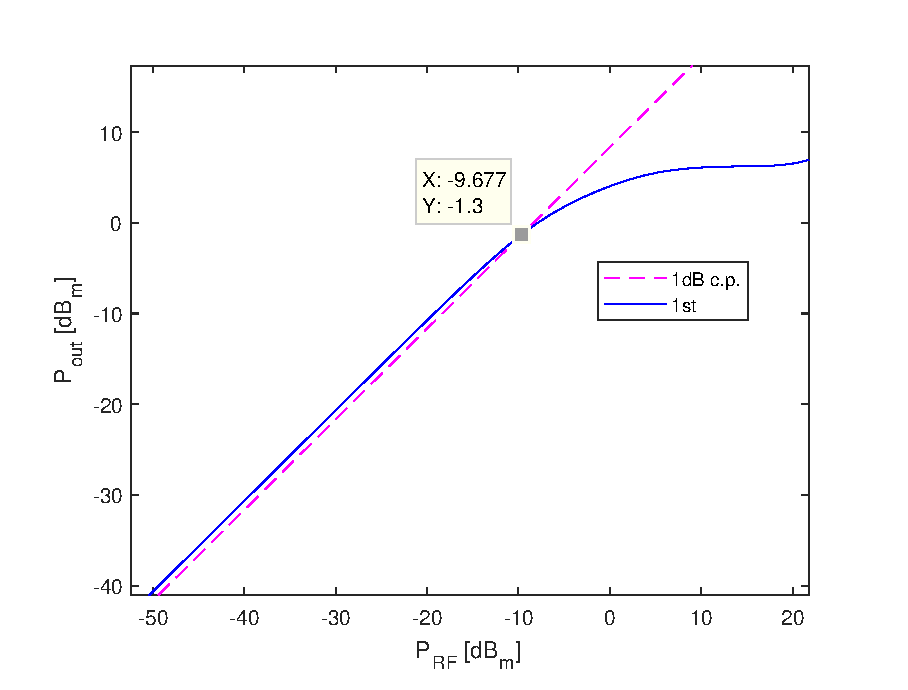
\includegraphics[scale=.7]{1dB_compression_2tone_layout}}
	\caption{1dB compression point, two tones.}
	\label{fig:1dB_2tones}
\end{figure}

\begin{figure}[H] 
	\centering
	\subfloat[][\emph{schematic}]{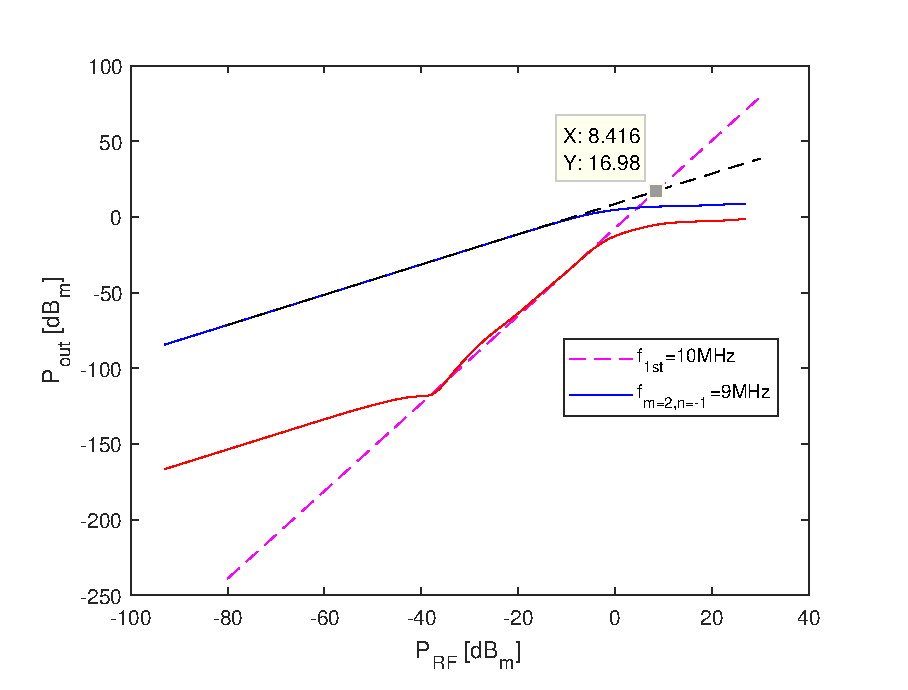
\includegraphics[scale=.7]{IIP3_schem_2tone}} \\
	\subfloat[][\emph{layout}]{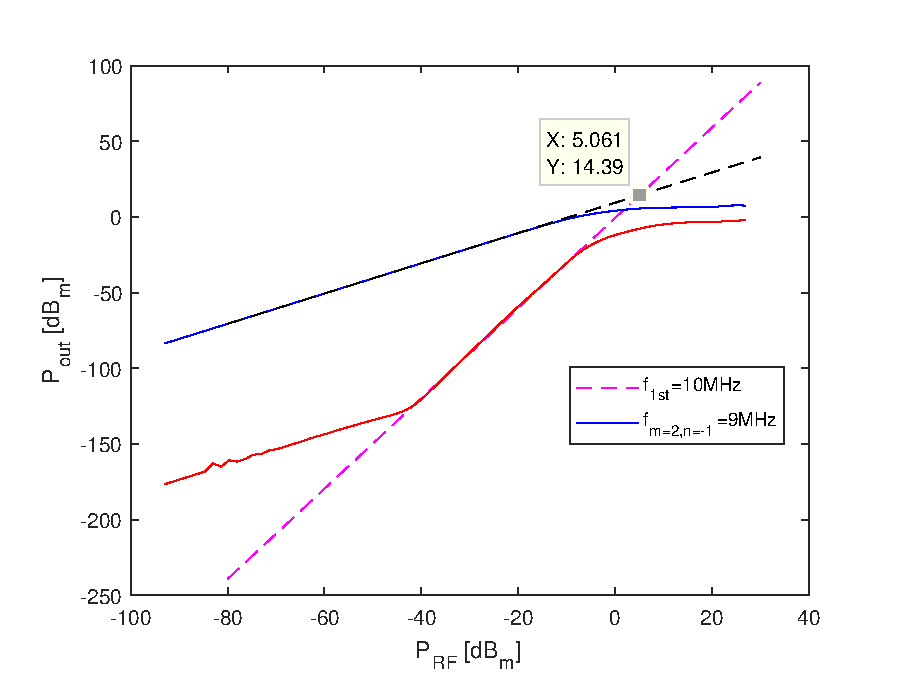
\includegraphics[scale=.7]{IIP3_layout_2tone}}
	\caption{Harmonics power, IIP\textsubscript{3} and IIP\textsubscript{5} in schematic, two tone analysis.}
	\label{fig:IIP3_2t_schem}
\end{figure}

\begin{figure}[H] 
	\centering
	\subfloat[][\emph{schematic}]{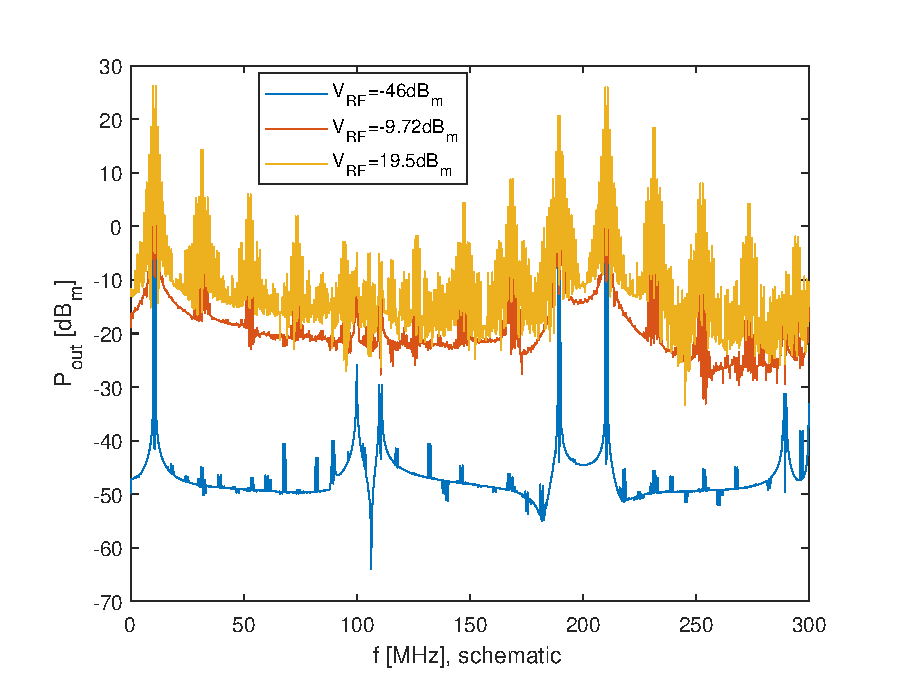
\includegraphics[scale=.7]{DFT_2tones_schem}} \\
	\subfloat[][\emph{layout}]{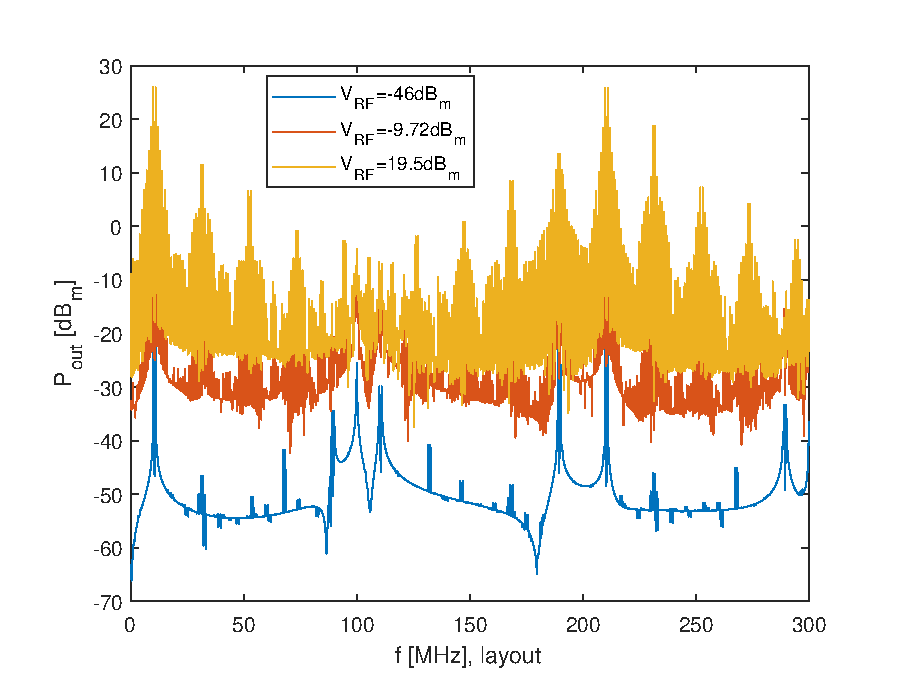
\includegraphics[scale=.7]{DFT_2tones_layout}}
	\caption{DFT, comparison between layout and schematic; cosine2 smoothing function.}
	\label{fig:DFT_2ton}
\end{figure}

\begin{figure}[H] 
	\centering
	\subfloat[][\emph{schematic}]{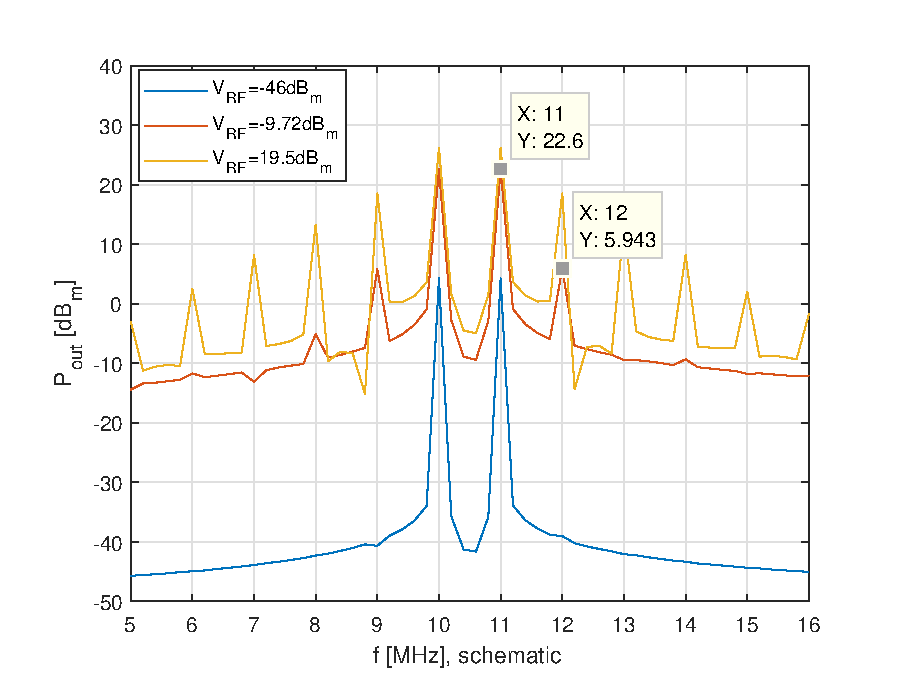
\includegraphics[scale=.7]{DFT_2tones_schem_zoom}} \\
	\subfloat[][\emph{layout}]{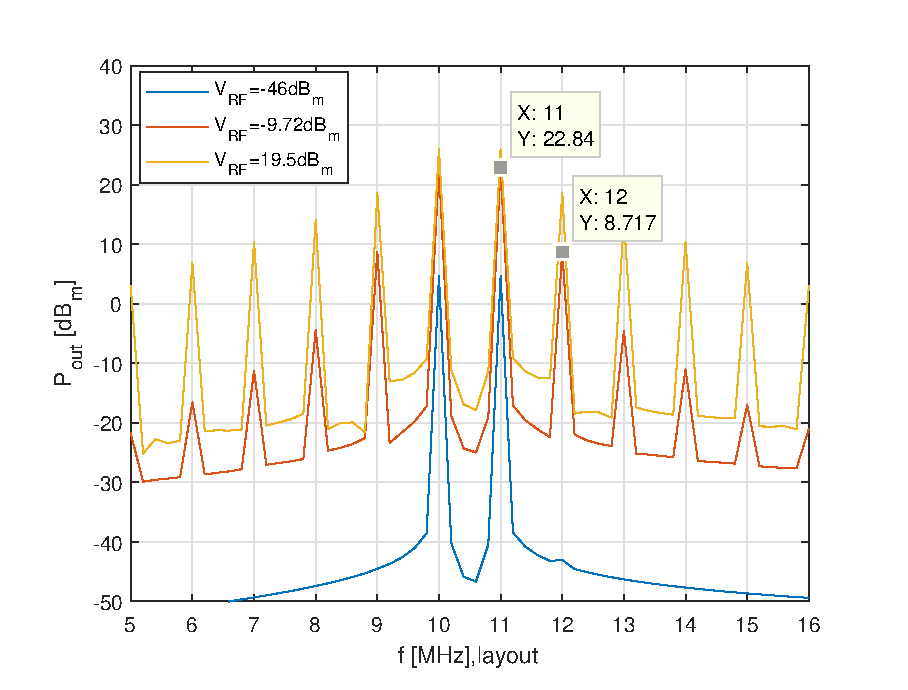
\includegraphics[scale=.7]{DFT_2tones_layout_zoom}}
	\caption{DFT, comparison between layout and schematic. CIM\textsubscript{3} measurement at 1dB compression point; cosine2 smoothing function. }
	\label{fig:DFT_2ton_zoom}
\end{figure}


\subsection{Bandwidth and CMRR of RF stage (output node filtering, current mixing)}
In order to have an estimation of what the maximum operating frequency of the mixer could be, an ac analysis on the differential RF stage has been made, keeping LO stage fixed in bias condition. The analysis led to the bode plot seen in \\FIGURA\\, which shows a \(-3dB\) bandwidth of approximately \(113MHz\), and a common mode rejection ratio of \\dB\\. Our assumptions on LO and RF frequencies were thus considered adequate, since represent the worst-case performances of the mixer. Moreover it has to be noticed that the mixing operation is done on the RF current. Maximum operating frequency could thus be improved reducing output node capacitance. 
\subsection{pavarotti?}
